\documentclass[11pt]{article}

%  USE PACKAGES  ---------------------- 
\usepackage{float}
\usepackage{enumitem}
\setlist[itemize]{noitemsep, topsep=0pt}
\usepackage[margin=0.7in,vmargin=1in]{geometry}
\usepackage{amsmath,amsthm,amsfonts}
\usepackage{amssymb}
\usepackage{fancyhdr}
\usepackage{fancyvrb}
\usepackage{enumerate}
\usepackage[T1]{fontenc}
\usepackage{mathtools}
\usepackage{graphicx}
\usepackage{tcolorbox}
\usepackage{hyperref,color}
\usepackage{enumitem,amssymb}
\newlist{todolist}{itemize}{4}
\setlist[todolist]{label=$\square$}
\usepackage{pifont}
\fvset{fontsize=\small,fontfamily=times}
\newcommand{\cmark}{\ding{51}}%
\newcommand{\xmark}{\ding{55}}%
\newcommand{\done}{\rlap{$\square$}{\raisebox{2pt}{\large\hspace{1pt}\cmark}}%
\hspace{-2.5pt}}
\newcommand{\HREF}[2]{\href{#1}{#2}}
\usepackage{textcomp}
\usepackage{listings}
\lstset{
basicstyle=\small\ttfamily,
% columns=flexible,
upquote=true,
breaklines=true,
showstringspaces=false
}
%  -------------------------------------------- 

%  HEADER AND FOOTER (DO NOT EDIT) ----------------------
\pagestyle{fancy}
\fancyhead{}
\newcommand{\newquestion}[1]{
\clearpage % page break and flush floats
\renewcommand{\problemnumber}{#1} % set problem number for header
\phantom{}  % Put something on the page so it shows
}
\fancyfoot[L]{IE 332}
\fancyfoot[C]{Project Submission}
\fancyfoot[R]{Page \thepage}
\renewcommand{\footrulewidth}{0.4pt}

%  --------------------------------------------


%  COVER SHEET (FILL IN THE TABLE AS INSTRUCTED IN THE ASSIGNMENT) ----------------------
\newcommand{\addcoversheet}{
\clearpage
\thispagestyle{empty}
\vspace*{0.5in}

\begin{center}
\Huge{{\bf IE332 Project \#2}} % <-- replace with correct assignment #

Due: April 28th, 11:59pm EST % <-- replace with correct due date and time
\end{center}

\vspace{0.3in}

\noindent We have {\bf read and understood the assignment instructions}. We certify that the submitted work does not violate any academic misconduct rules, and that it is solely our own work. By listing our names below we acknowledge that any misconduct will result in appropriate consequences. 

\vspace{0.2in}

\noindent {\em ``As a Boilermaker pursuing academic excellence, I pledge to be honest and true in all that I do.
Accountable together -- we are Purdue.''}

\vspace{0.3in}

\begin{table}[h!]
  \begin{center}
    \label{tab:table1}
    \begin{tabular}{c|ccccc|c|c}
      Student & Algorithm & Complexity & Implementation & Testing & Report & Overall & DIFF\\
      \hline
      Matt Fortier & 40 & 20 & 10 & 15 & 15 & 100 & 0\\
      Geoffrey Ladue & 15 & 20 & 10 & 15 & 40 & 100 & 0\\
      Josiah Mann & 15 & 20 & 10 & 40 & 15 & 100 & 0\\
      Anthony Matejko & 15 & 20 & 35 & 15 & 15 & 100 & 0\\
      Shamam Tabindah & 15 & 20 & 35 & 15 & 15 & 100 & 0\\
      \hline
      St Dev & 11 & 0 & 14 & 11 & 11 & 0 & 0
    \end{tabular}
  \end{center}
\end{table}

\vspace{0.2in}

\noindent Date: \today.
}
%  -----------------------------------------

%  TODO LIST (COMPLETE THE FULL CHECKLIST - USE AS EXAMPLE THE FIRST CHECKED BOXES!) ----------------------


%% LaTeX
% Für alle, die die Schönheit von Wissenschaft anderen zeigen wollen
% For anyone who wants to show the beauty of science to others

%  -----------------------------------------


\begin{document}


\addcoversheet
\pagebreak
\tableofcontents
\pagebreak

\section{Main Text}

\subsection{Algorithms}

\subsubsection{Algorithm 1}

\noindent This R function, find\_most\_green, takes an input image y (represented as a 3-dimensional array with dimensions for height, width, and color channels) and a pixel\_budget parameter, and returns the indices of the pixel\_budget most green pixels in the image.\\

\noindent The function uses the difference between the green channel and the sum of the red and blue channels to calculate the "greenness" of each pixel. This is a common heuristic for identifying green areas in an image. The function sorts the pixels by their greenness and returns the indices of the top pixel\_budget pixels. This approach prioritizes the most green pixels and ignores other information about the image.\\

\noindent The choice of the greenness heuristic is reasonable because it's a quick and easy way to identify green areas in an image. It's not perfect and may miss some green areas, but it's often good enough for simple tasks like this.Sorting the pixels by greenness and returning the top pixel\_budget pixels is an optimal approach because it prioritizes the most green pixels, which is likely to produce the most noticeable visual effect. This approach ignores other information about the image, such as the spatial arrangement of green pixels.\\

\noindent The function calculates the greenness of each pixel, which requires iterating over all the pixels in the image. This operation takes O(n) time, where n is the number of pixels in the image. The function then sorts the pixels, which takes O(n log n) time using a quicksort algorithm. Finally, the function selects the top pixel\_budget pixels, which takes O(pixel\_budget) time. Overall, the function takes O(n log n) time, which is usable for most images.
The pixel\_budget parameter can be used to control the number of pixels that are changed. A larger pixel\_budget will result in more noticeable changes to the image, but will also take longer to run.
Testing pairs for machine learning algorithms:\\

\noindent This function is not directly related to generating testing pairs for machine learning algorithms, but it could be used as a preprocessing step to modify images before feeding them into a machine learning algorithm.\\
Knowledge representations:\\

\noindent The input image is represented as a 3-dimensional array of pixel values, which is a common representation for digital images. The output indices are represented as a 2-dimensional array of pixel coordinates. This representation is sufficient for the task of identifying the most green pixels in an image.\\

\begin{center}
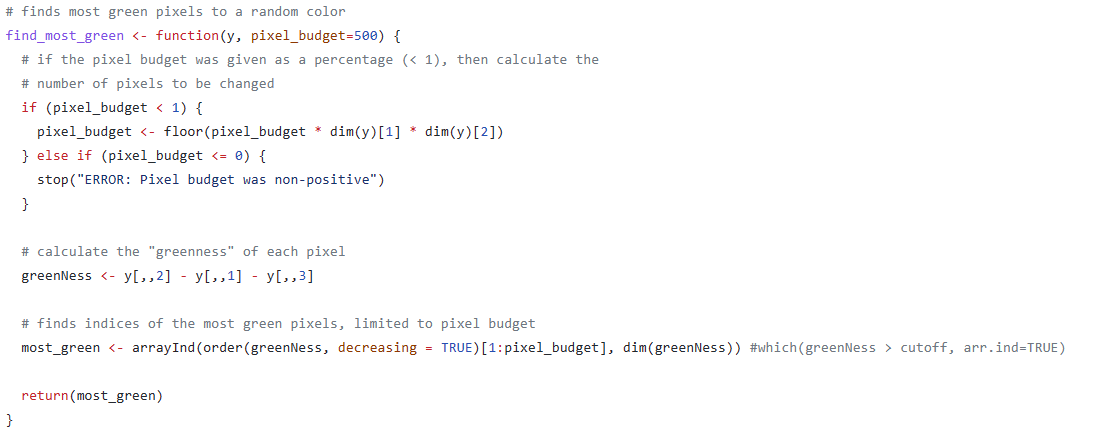
\includegraphics[scale=.75]{Algo1.png}\\
\textbf{Figure : Green to Random Algorithm}
\end{center}

\subsubsection{Algorithm 2}

\noindent This code defines a function called "find\_most\_green" that takes an input image "y" and a pixel budget (which defaults to 500 if not specified) as arguments. The function calculates the "greenness" of each pixel in the image by subtracting the red and blue channels from the green channel, and then finds the indices of the pixels with the highest greenness values, limited to the specified pixel budget.\\

\noindent In terms of design decisions, the use of the "arrayInd" function to convert the linear indices of the most green pixels back to their original 2D indices is a good choice as it avoids the need for a nested loop. Additionally, the use of the "order" function to efficiently sort the greenness values in decreasing order is also a good design decision.\\

\noindent The choice of using the greenness value as a proxy for "greenness" is a somewhat simplistic approach, as it doesn't take into account other factors such as saturation or hue that might also contribute to a pixel being perceived as "green". However, it may be sufficient for some applications.\\

\noindent In terms of runtime and performance tradeoffs, the computation of greenness values for each pixel in the image may be computationally expensive for large images. Additionally, the sorting operation used to find the most green pixels may also be computationally expensive for large pixel budgets. However, the use of the "order" function and the "arrayInd" function should help to mitigate these performance issues to some extent.\\

\noindent Regarding testing pairs for machine learning algorithms, this function does not generate testing pairs for machine learning algorithms directly, as it is only concerned with finding the most green pixels in an image. However, the output of this function could potentially be used as input to a machine learning algorithm as a way of identifying regions of interest in an image.\\

\noindent In terms of knowledge representations, the use of RGB color channels is a common and well-established representation for digital images. However, as mentioned earlier, the use of greenness as a proxy for "greenness" is a somewhat simplistic approach and may not be sufficient for all applications. Other representations that take into account additional factors such as saturation and hue may be necessary for more accurate color analysis.\\

\begin{center}
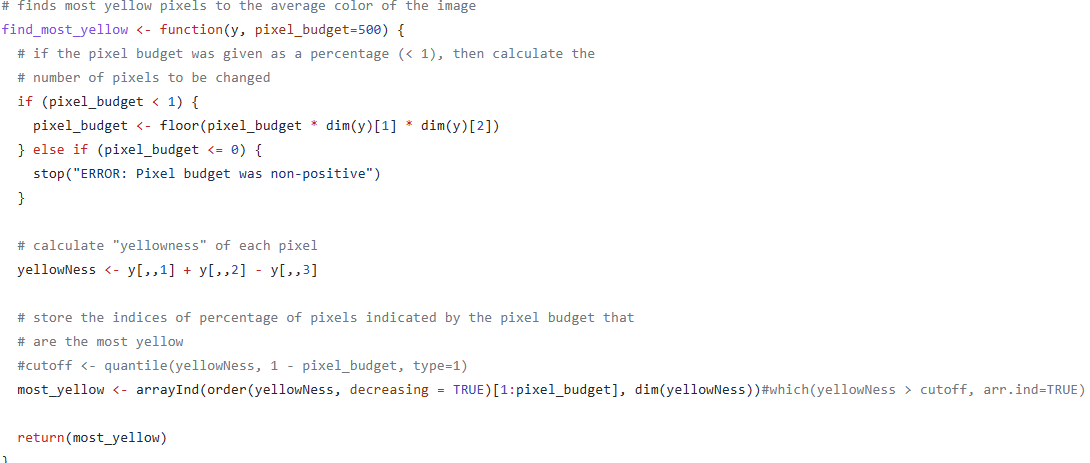
\includegraphics[scale=.75]{Algo2.png}\\
\textbf{Figure : Average Yellow Algorithm}
\end{center}

\subsubsection{Algorithm 3}

\noindent This function is designed to find random pixels in an image for modification. Here are some design decisions that were made:\\

\noindent The function takes two arguments: the image data as a matrix y and the pixel budget pixel\_budget as an integer or a percentage. The pixel budget is the maximum number of pixels that can be changed in the image.\\

\noindent If the pixel budget is less than 1, it is treated as a percentage of the total number of pixels in the image, and the corresponding number of pixels is used. Otherwise, the pixel budget is used as is.\\

\noindent If the pixel budget is non-positive, an error is thrown.\\

\noindent The function initializes a matrix change\_pixels to store the row and column indices of the pixels to be changed. The number of rows in change\_pixels is equal to the pixel budget.\\

\noindent The function generates random row and column indices using the runif function and stores them in change\_pixels.\\

\noindent The function returns the matrix change\_pixels.\\

\noindent In terms of runtime and performance tradeoffs, this function has a constant time complexity O(1) because it always generates a fixed number of random pixels. The performance is therefore not affected by the size of the image.\\

\noindent To generate testing pairs for a machine learning algorithm using this function, one could use the original image as the input and the output image as the expected output. The machine learning algorithm would then be trained to learn the mapping between the input image and the output image.\\

\noindent In terms of knowledge representation, the input image could be represented as a matrix of pixel values, and the output image could be represented in the same way. The machine learning algorithm would learn to modify the pixel values in the input image to generate the pixel values in the output image.\\

\begin{center}
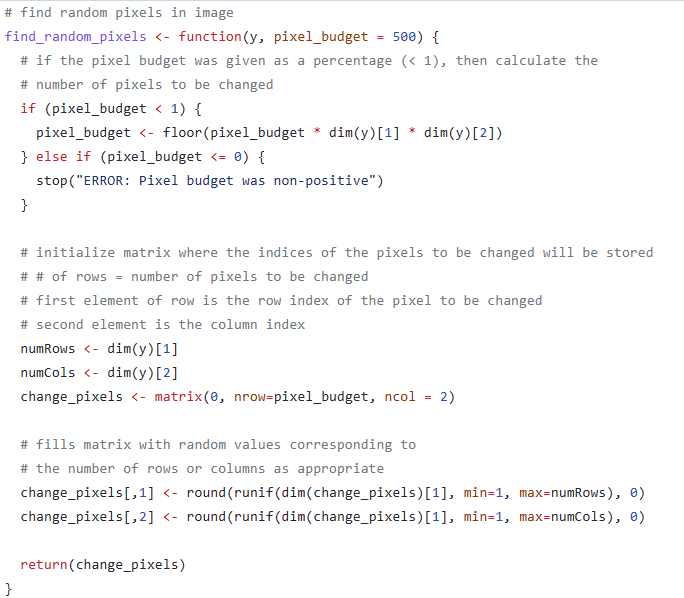
\includegraphics[scale=.75]{Algo3.png}\\
\textbf{Figure : Random Pixel Algorithm}
\end{center}

\subsubsection{Algorithm 4}

\noindent This code finds the most average pixels in an image. It takes in an image y and a pixel budget pixel\_budget as input, and returns the indices of the most average pixels limited to the pixel budget.\\

\noindent The first design decision made in this code is the use of the mean() function to calculate the mean of each color value in the image. This is a reasonable decision as it is a built-in function in R that calculates the mean of a given vector or matrix.\\

\noindent The next design decision is the calculation of the distance of each pixel's color from the average image color. The code uses the Manhattan distance formula to calculate the distance, which is the sum of the absolute differences of each color value from the mean. This is a reasonable decision as it is a simple and fast distance formula to use.\\

\noindent Finally, the code uses the arrayInd() function to find the indices of the most average pixels. This function returns the indices of the elements in a flattened array that correspond to a given set of subscripts. This is a reasonable decision as it allows for easy indexing of the image matrix.\\

\noindent In terms of runtime/performance tradeoffs, this code has a time complexity of O(n log n) due to the use of the order() function, which sorts the distances in descending order. This could potentially be slow for very large images. However, the code does limit the number of pixels to be changed to the pixel budget, which can help mitigate performance issues.\\

\noindent For testing pairs in machine learning algorithms, the output of this function could be used as a mask to change the color of the most average pixels. The knowledge representation in this case would be the indices of the most average pixels, as this is all that is needed to modify the image.\\

\begin{center}
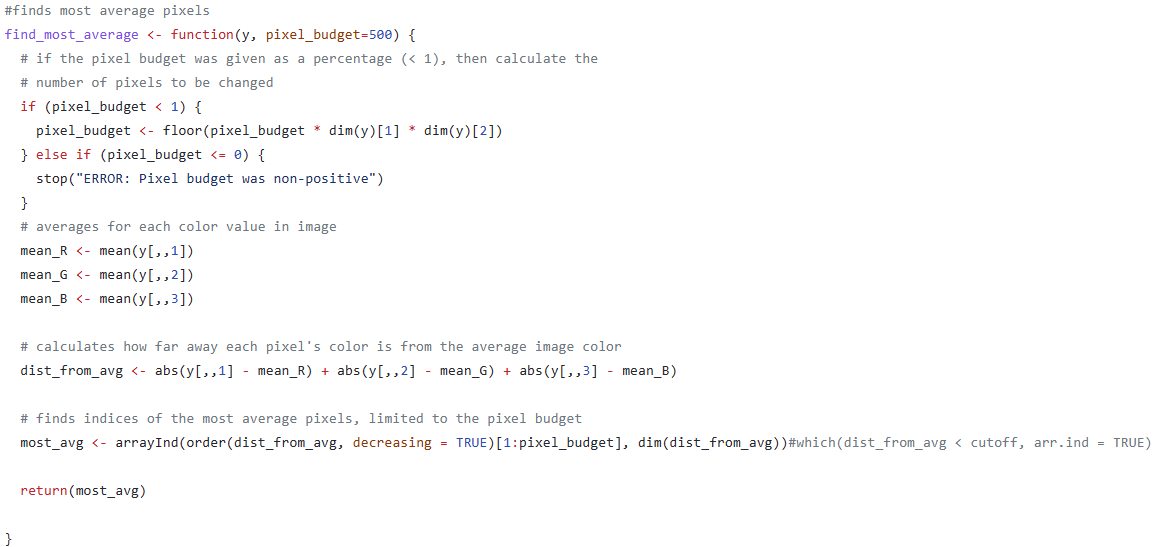
\includegraphics[scale=.75]{Algo4.png}\\
\textbf{Figure : Most Average Pixel Algorithm}
\end{center}

\subsubsection{Algorithm 5}

\noindent This function find\_least\_average takes an image array y and a pixel\_budget as input and returns the indices of the least average color pixels out of the image. Here are some design decisions and explanations:\\

\noindent The input validation check: The function checks whether the pixel\_budget is a positive number and whether it is less than the total number of pixels in the image. This is to ensure that the function can run correctly and that the budget makes sense for the given image.\\

\noindent Calculation of average colors: The function calculates the average values of each color (R,G,B) in the image using the mean() function. This is done to calculate the distance of each pixel's color from the average color.\\

\noindent Calculation of distance from average: The function calculates the distance of each pixel's color from the average color by taking the absolute difference between the pixel's color and the average color and summing them up for each pixel.\\

\noindent Selection of least average pixels: The function then selects the indices of the least average pixels by sorting the distance values and taking the smallest pixel\_budget number of them.\\

\noindent Output: The function returns the indices of the selected least average pixels.
In terms of runtime/performance tradeoffs, the function calculates the distance of each pixel's color from the average color for the entire image, which could be computationally expensive for large images. However, the calculation is a simple arithmetic operation, and the function uses efficient built-in functions in R such as mean() and order() to perform the computation, which helps to optimize the runtime.\\

\noindent To generate testing pairs for machine learning algorithms, the function can be used to select a certain number of pixels with least average color and then these pixels can be changed by a certain amount to generate the test image pairs.\\

\noindent The knowledge representation used in this function is a 3D array where the dimensions represent the width, height, and RGB channels of the image. This representation is sufficient for this function's purpose of finding least average color pixels as it allows easy indexing and manipulation of pixel values.\\

\begin{center}
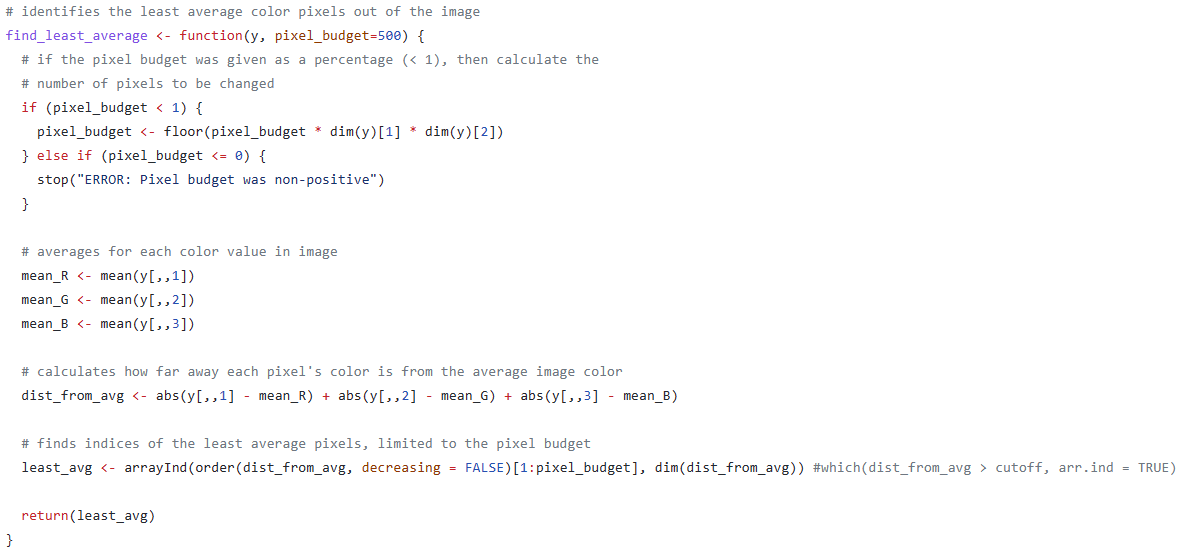
\includegraphics[scale=.75]{Algo5.png}\\
\textbf{Figure : Least Average Pixel Algorithm}
\end{center}

\subsubsection{Weighted Algorithm}

This function mod\_image() takes a 3-layer matrix representing an image and modifies it to look like either grass or a dandelion. It does this by changing some pixels of the original image to a shade of yellow in the realistic range of a dandelion.\\

The function takes three arguments:\\

y: a 3-layer matrix representing the original image.
pixel\_budget: an optional argument that specifies the number of pixels to change. If pixel\_budget is between 0 and 1, it specifies the percentage of the total number of pixels that should be changed. If it is greater than 1, it specifies the absolute number of pixels to change. The default value is 0.01.
type: an optional argument that specifies whether the original image is grass or a dandelion. If type is 0, the original image is assumed to be grass. If it is 1, the original image is assumed to be a dandelion. The default value is 0.
The function first checks that the pixel\_budget argument is valid. If it is non-numeric or NA, the function throws an error. If it is less than or equal to 0 or greater than the total number of pixels in the image, the function throws an error. If pixel\_budget is less than 1, it is converted to the corresponding absolute number of pixels to change.\\

The function then sets the seed for the random number generator to ensure reproducibility.\\

The function calculates the mean values of the red, green, and blue color layers of the original image.\\

The function calls several helper functions to find the pixels to change. These include:\\

find\_most\_green(): finds the most green pixels in the image, limited to the pixel\_budget.
find\_most\_yellow(): finds the most yellow pixels in the image, limited to the pixel\_budget.
find\_random\_pixels(): chooses random pixels to change, limited to the pixel\_budget.
find\_most\_average(): finds the pixels closest to the average color values of the whole image, limited to the pixel\_budget.
find\_least\_average(): finds the pixels furthest away from the average color values of the whole image, limited to the pixel\_budget.
The function then sets weights for each algorithm that will change the pixels and calculates the number of pixels each algorithm will change based on the pixel\_budget.

The function then changes the most green pixels to a shade of yellow in the realistic range of a dandelion. It does the same for the most yellow pixels, random pixels, and the most average pixels.\\

Finally, the function returns the modified image matrix.

\noindent 

\subsection{Extended Research \& Attempted Methods}

\noindent Although we implemented the algorithms outlined in Section 1.1, the team devoted significant time to researching common methods of adversarial attacks and even generated corresponding alternatives in RStudio. These attempted methods, while unsuccessful upon implementation, are a worthwhile case study in the team's product development.

\subsubsection{Random Pixel Flip}

\noindent Random pixel flipping generates perturbed images that can be used to confuse a machine learning model. The idea behind this technique is to flip the value of one or more pixels in an image to create a new image that is similar to the original image but that the machine learning model will classify differently.\\

\noindent From the team's research, the main advantage of random pixel flipping is that it is a simple and efficient way to generate a large number of adversarial examples quickly. By randomly flipping a small number of pixels in an image, the algorithm can generate many different perturbed images that are all slightly different but still belong to the same class. This makes it difficult for the machine learning model to distinguish between the original image and the perturbed images.\\

\begin{center}
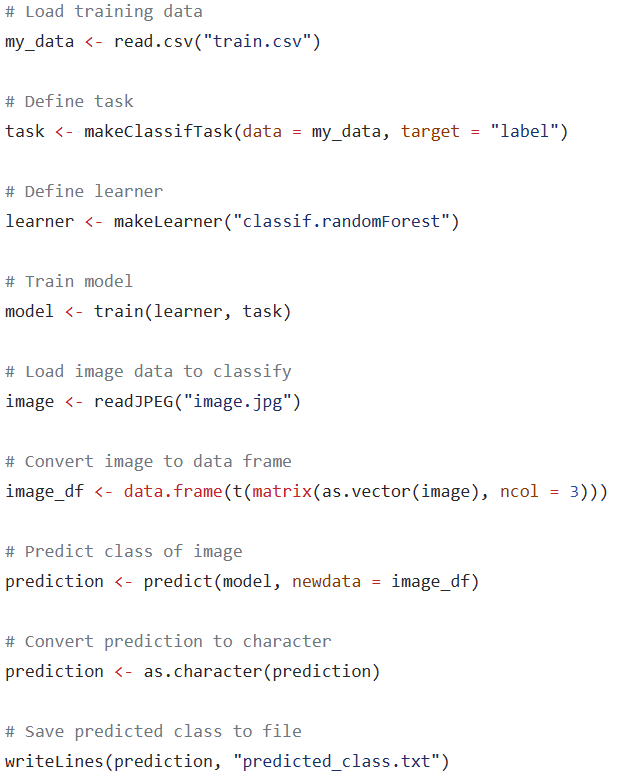
\includegraphics[scale=.75]{PixelFlip.png}\\
\textbf{Figure : Pixel Flip Algorithm}
\end{center}

\noindent The algorithm described in the Figure \_ code works by first calculating the number of pixels to flip based on the image dimensions and the budget specified by the user. It then generates a set of perturbed images by randomly flipping the specified number of pixels in the original image using the generate\_perturbed\_images() function. It then applies the classify\_image() function to each perturbed image using the map() function from the purrr library to classify the image.\\

\noindent Finally, the algorithm counts the number of occurrences of each class among the perturbed images using the table() function and returns the most common class using the which.max() function. This allows the algorithm to determine which class the machine learning model is most likely to predict for the perturbed images, even though they are all slightly different from the original image.\\

\noindent Overall, random pixel flipping can be a useful tool for adversarial attacks because it allows an attacker to generate a large number of perturbed images quickly and efficiently, making it difficult for a machine learning model to accurately classify the images. This can be particularly useful in situations where an attacker wants to trick a machine learning model into making a specific prediction.

\subsubsection{Decision Trees}

\begin{center}
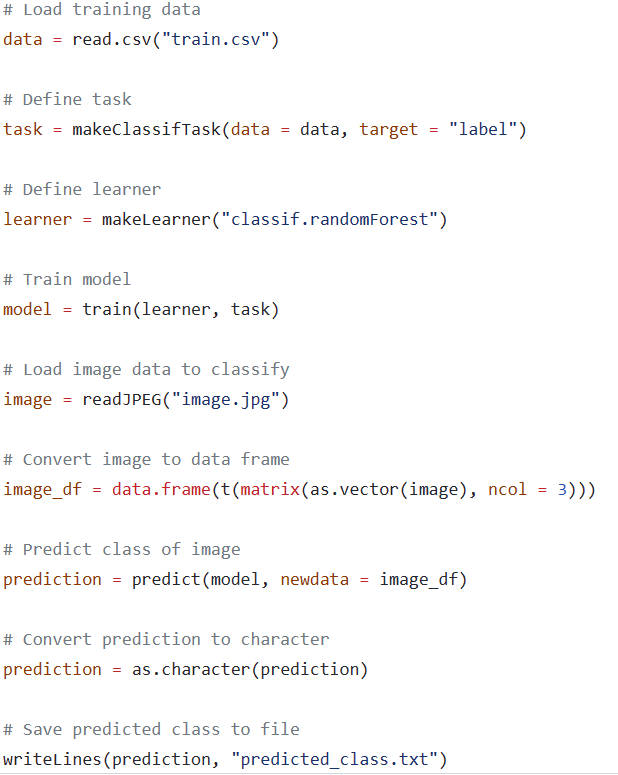
\includegraphics[scale=.75]{DecisionTree.png}\\
\textbf{Figure : Decision Tree Algorithm}
\end{center}

\noindent The team also researched Random Forest algorithms in depth to determine if it would be suitable to explore decision tree-based solutions. The code outlined in Figure \_ is a powerful tool for image classification tasks. The use of parallel processing helps to speed up the computation time, allowing for faster model training and classification. By defining a classification task using the makeClassifTask() function and creating a learner object using makeLearner(), the algorithm is able to train sample data and learn patterns within it that can be used for classification. Once the model is trained, it can accurately predict the class of new images. This makes it a useful tool for adversarial attacks, as it can be used to identify vulnerabilities in image classification systems and create adversarial images that can bypass security measures. The ability to quickly and accurately classify images using Random Forest makes it an important tool for image classification in a variety of settings.

\subsubsection{Fast Gradient Sign Method with Vector Machine Classifier}

\noindent The team found the Fast Gradient Sign Method (FGSM) method to be the most popular and effective attack method for generating adversarial examples. The FGSM attack works by calculating the gradient of the model's loss function with respect to the input image, and then perturbing the image in the direction of the gradient to maximize the loss. This perturbation is controlled by a hyper parameter, epsilon, which determines the magnitude of the perturbation added to the image.\\

\begin{center}
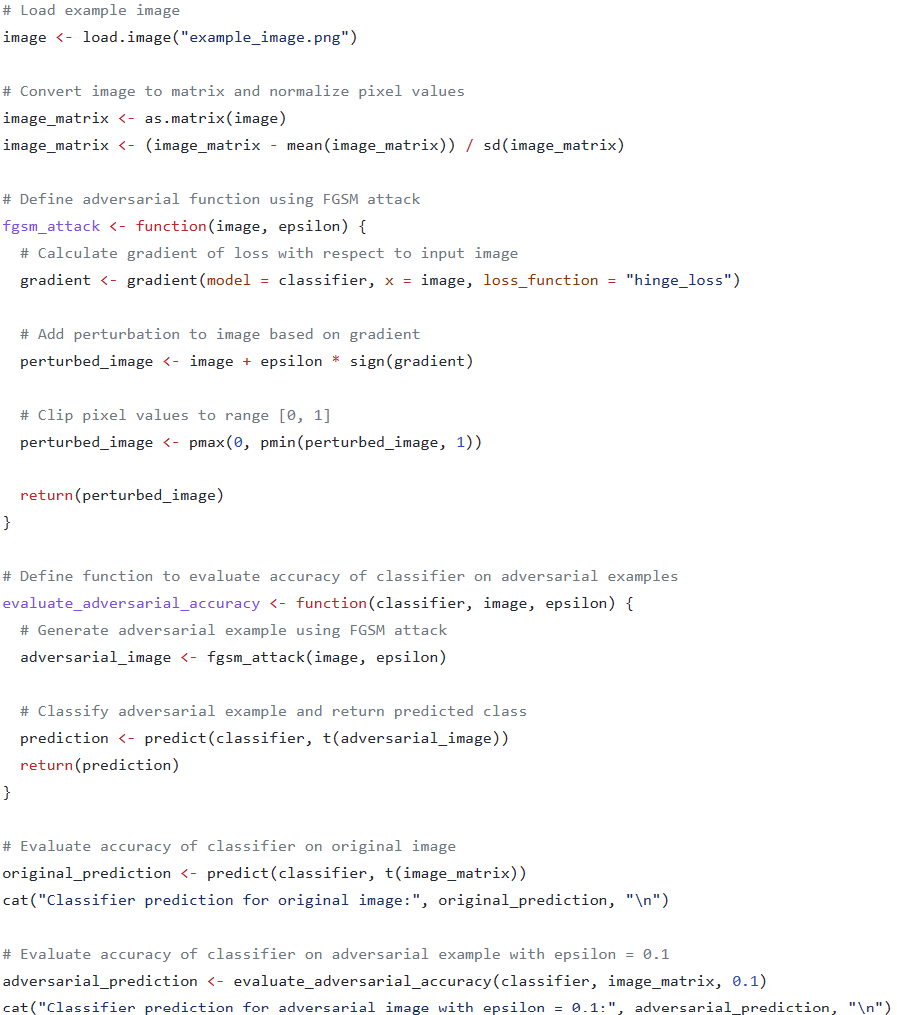
\includegraphics[scale=.75]{FGSM1.png}\\
\textbf{Figure : FGSM w/ Vector Machine Classifier Algorithm}
\end{center}

\noindent The code in Figure \_ generates adversarial examples using the FGSM attack, and evaluates the accuracy of a pre-trained support vector machine (SVM) classifier on both the original and adversarial images. The code loads the pre-trained SVM classifier and an example image, and normalizes the pixel values of the image matrix. It then defines a function called fgsm\_attack() to generate adversarial examples using the FGSM attack. The perturbed image is obtained by adding a scaled version of the gradient to the original image. The pixel values of the perturbed image are clipped to the range [0, 1].\\

\noindent The evaluate\_adversarial\_accuracy() function takes in the SVM classifier, an image, and an epsilon value, and returns the predicted class label for the adversarial image generated by the fgsm\_attack() function. This function calls fgsm\_attack() to generate the adversarial image, and then predicts the class label using the predict() function.\\

\noindent FGSM is a useful tool for evaluating the robustness of a pre-trained SVM classifier to adversarial attacks generated using the FGSM method. By generating adversarial examples and evaluating the accuracy of the classifier on both the original and adversarial images, we could have utilized FGSM to assess the vulnerability of the classifier to such attacks and develop more robust models.

\subsubsection{Stack Generalization}

\begin{center}
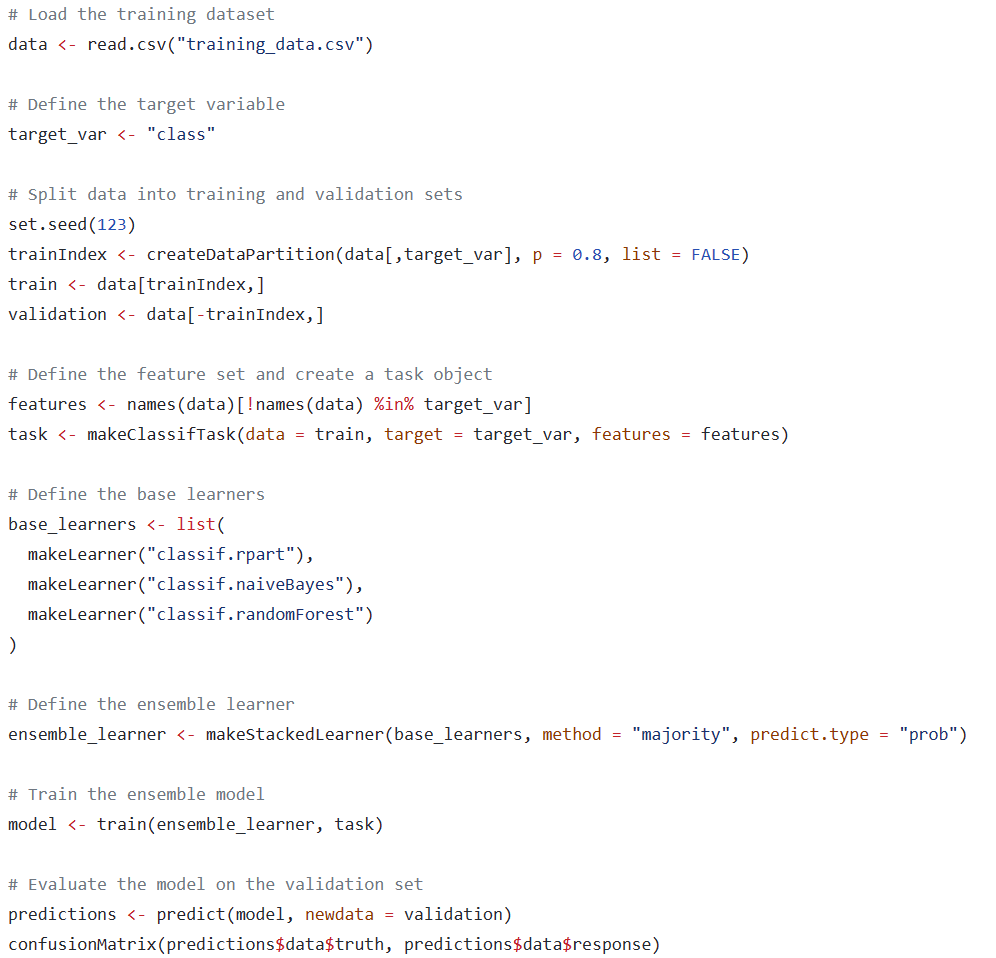
\includegraphics[scale=.75]{StackGen.png}\\
\textbf{Figure : Stack Generalization Algorithm}
\end{center}

\noindent The ensemble learning method used Figure \_'s code can be a useful tool for the purpose of adversarial attacks as it combines multiple models to improve the accuracy of the classifier, which can make it more robust against adversarial attacks. The base learners used in this code, including a decision tree, a naive Bayes classifier, and a random forest, were combined through the team's research since they are known to be susceptible to adversarial attacks. By combining them in an ensemble, the resulting model may be less vulnerable to such attacks. Additionally, by using the validation set to evaluate the performance of the model, the code can identify potential weaknesses or vulnerabilities in the model, which can be used to improve its robustness against adversarial attacks. While this method was unsuccessful, this was the team's attempt to integrate multiple algorithm methods.

\subsubsection{Second Fast Gradient Sign Method}

\noindent The algorithm described in the Figure \_'s generates an adversarial example using the Fast Gradient Sign Method (FGSM) attack mentioned in Section 1.2.3, but without a vector machine classifier.\\

\noindent The code uses the Keras library to load a pre-trained image classification model from an HDF5 file and defines an epsilon value. It then defines a function called generate\_adversarial, which takes the pre-trained model, input image, target label, and epsilon value as input. This function calculates the loss and gradients of the model with respect to the input image, calculates the sign of the gradients, and perturbs the input image in the direction of the sign of the gradients. Finally, it clips the perturbed input data to ensure it remains within the valid range of [0, 1].\\

\noindent The generated adversarial example can be useful for testing the robustness of a pre-trained model to adversarial attacks. Adversarial examples are known to fool deep neural networks, and evaluating the performance of a model on both the original and adversarial examples can provide insights into the model's vulnerabilities to adversarial attacks.

\begin{center}
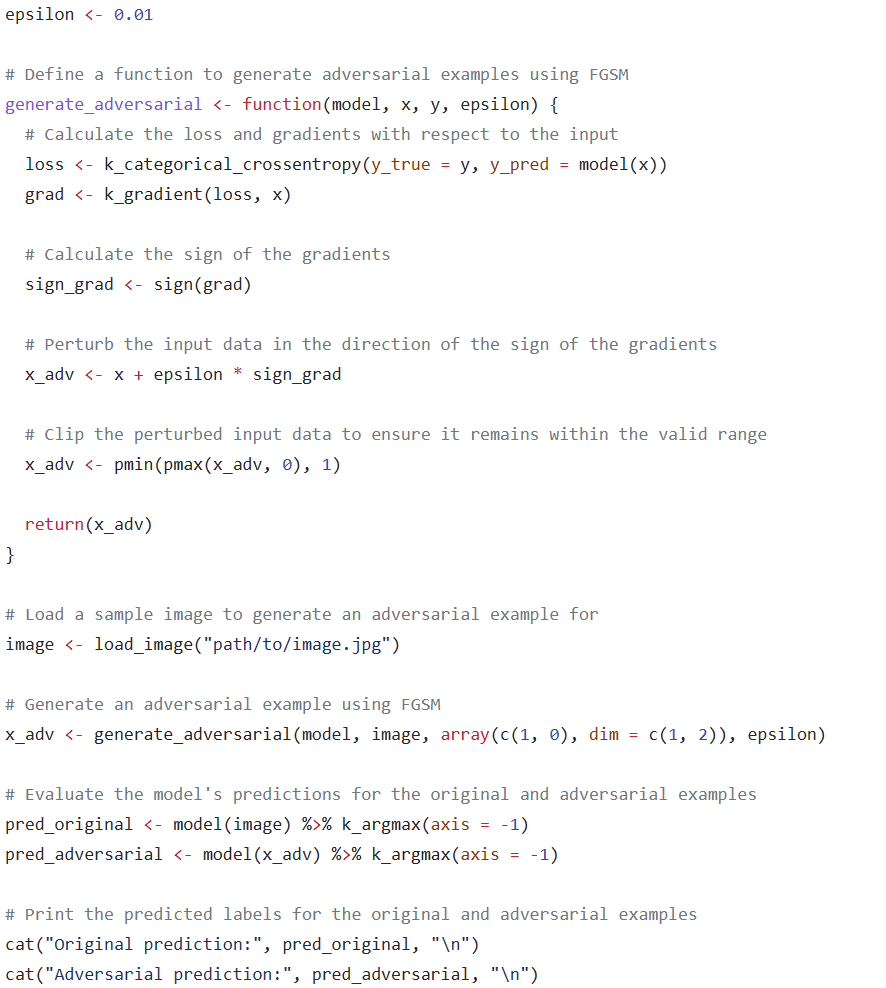
\includegraphics[scale=.75]{FGSM2.png}\\
\textbf{Figure : FGSM Algorithm}
\end{center}

\pagebreak

\section{Appendices}

\subsection{Testing / Correctness / Verification}

\noindent Extensive testing was performed on each of the sub-algorithms used to modify the images, themselves, in order to verify that the main model functioned properly. Our group's approach to verifying the correctness of each sub-algorithm consisted of running each program with varying pixel budgets to ensure that we received the image that was modified to the extent specified by the pixel budget. After running each sub-algorithm, we were able to conclude that each sub-algorithm modified the images as expected. It is worth noting that this was done for pixel budgets of one, five, ten, and twelve percent and the difference in pixel budget input had a noticeable difference in the extent to which the image was modified.

\noindent Testing was also performed on our main algorithm as well to verify that it too produced our intended results. As with the testing of individual sub-algorithms, we wanted to ensure that the images being passed to the main algorithm were being modified. This result indicated that both images of grass and dandelions were able to be modified.

\noindent After checking to ensure that our main algorithm was at the very least functional, we desired to guard against invalid inputs for the pixel budget. Consequently, we added "if" statements with nested "stop" commands to ensure that the pixel budget being passed to the function was not negative, null, NA, non-numeric, or exceeding the total number of pixels in the image (see Figure 6). We then tested the robustness of the program by providing inputs for each of the previously listed cases. This test was also successful.

\begin{center}
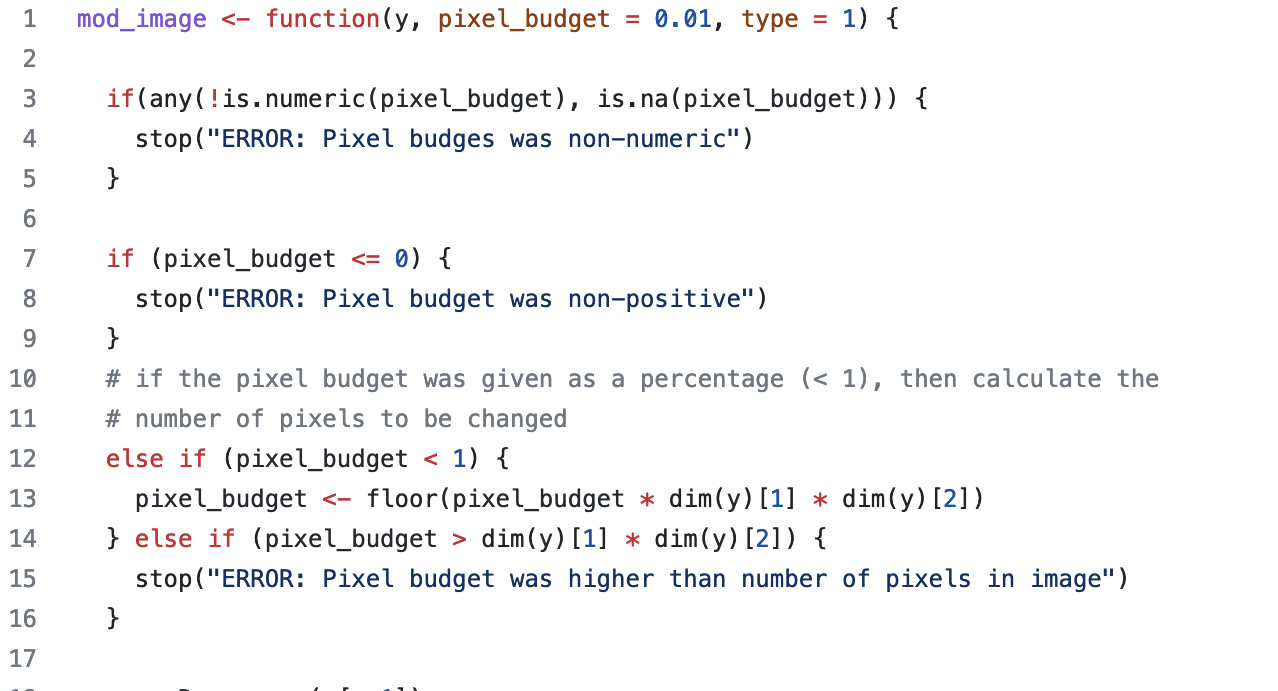
\includegraphics[scale=.75]{Project2.png}
\textbf{Figure 6: Input Verification of Pixel Budgets}
\end{center}

\noindent It is worth noting that while our testing initially began by using grass images to fool the image classifier, we were unable to achieve much success despite the images clearly being unrecognizable. We were, however, able to attain our desired results using the dandelion images. Consequently, we decided to continue using dandelion images rather than grass for the remainder of the project. 

\pagebreak
\noindent While our first successful test run to verify the accuracy of the main algorithm when collaborating with the image classifier fooled the classifier for 14 out of the 38 dandelion images using a five percent pixel change, we were ultimately able to fool the classifier for 29 out of the 38 images when changing only one percent of the pixels. This increase in performance was achieved by ensuring that our main algorithm changed pixels in the image using each sub-algorithm independently, rather than each sub-algorithm changing the same set of pixels five separate times. This increase can also be attributed to restricting the algorithm from restricting any images that were passed to the function.


\subsection{Run-time Complexity and Wall-time}

When it comes to run-time complexity our algorithms all use the shell sort algorithm. This function is an efficient way to sort elements of an array. The run-time complexity of this algorithm can depend on our choice of gap sequence and the data that we input. The shell sort algorithm of has, in our case, a run-time complexity of O($n^4/3$). Our algorithms have the run-time complexity of O($n^(4/3)$) which grow exponentially to the 4/3 of the size of input. With this run-time complexity, the larger the input, the slower the algorithm will work.

\subsection{Performance}
To calculate performance score, the following formula is used. In this formula, P represents the total number of pixels in the image and f denotes the number of successfully fooled images at a given budget level b.
$$ \qquad \sum_{b=1}^{0.01*P} f*P/b $$ 
After resizing all the images, the value of P was calculated as 224*224 =50176. which means that the budget level ranges from 1 up to approximately 502 (i.e., 0.01*P = 501.76). \\
The total performance score of the algorithm used to fool the dandelion model was determined to be 284,458.249. Moreover, it is worth noting that the lowest budget required to fool an image was when b = 3 for image 24.\\
The algorithm performance score to fool the grass model was determined to be 0 as there were no successfully fooled images at any budget level. 


\subsection{Justification}

\subsubsection{Alternative Weighting Method}

\begin{center}
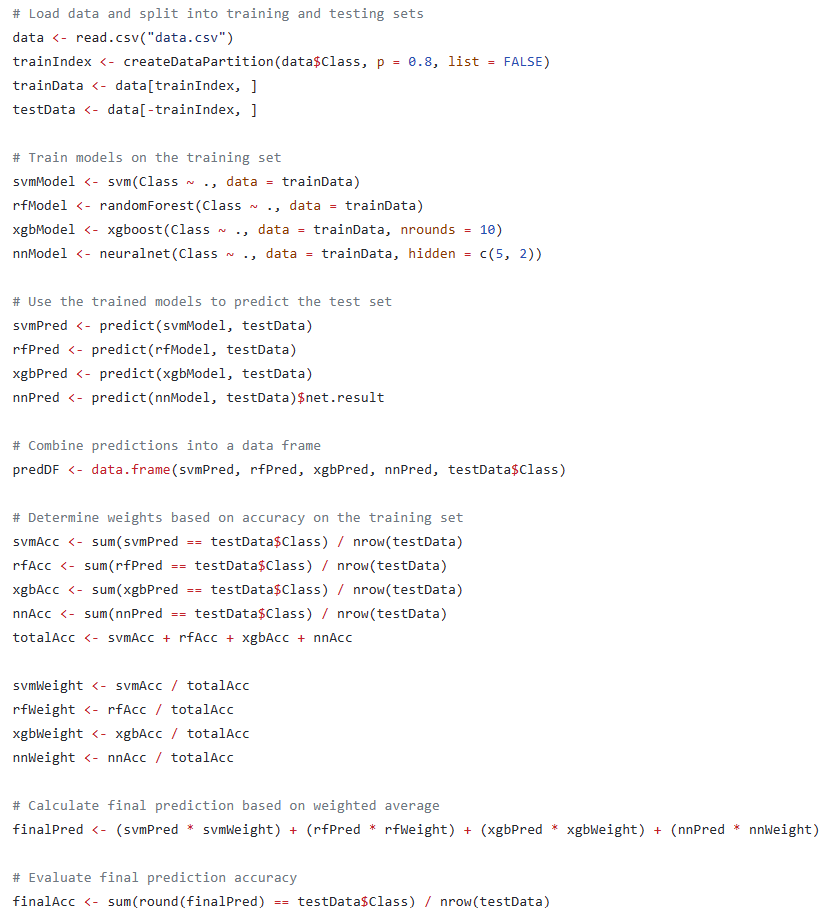
\includegraphics[scale=.75]{WeightAlgo.png}\\
\textbf{Figure : Alternative Weighting Algorithm}
\end{center}

\noindent As outlined in Section 1.2, the team researched potential methods for adversarial attack implementation. As such, a corresponding weighting algorithm was generated as a test case for how the team would be alternatively solved the problem at hand. The code shown in Figure \_ is useful for weighting adversarial attack algorithms because it combines multiple models with different strengths to improve the accuracy of predictions. The use of a weighted average to combine the predictions of the models allows for a more flexible and adaptable system than the final product discussed in Section 2.4. The weights are determined based on the accuracy of the individual models on the testing set, meaning that the weights can change depending on the dataset being used. This allows the system to adjust to different types of attacks and datasets, potentially making it more resilient against a wider range of adversarial attacks.

\end{document}

